\chapter{快照}

选择ROW方案,COW有难以克服的问题。

卷和快照的关系,是共存于一个物理卷、还是各自独立构成一个物理卷。
若独立占有一个物理卷,则打快照后,会改变卷ID,凡是依赖于这个信息的地方都需要进行适配。

索引的page cache

跨卷读,clone

参考产品
\begin{enumbox}
\item SheepDog/SSAN
\item Open VStorage
\item ***
\item FusionSorage
\item NetApp WALFS
\item Dell SC Series
\item 阿里云ECS
\item ***
\item SPDK
\item QEMU qcow2
\end{enumbox}

ROW设计问题
\begin{enumbox}
\item 在哪一层实现ROW
\item 链式快照和树状快照
\item COW里卷上有完整数据,快照有增量数据。
\item ROW第一次快照有全量数据,后续快照和卷无完整数据。ROW很自然地体现了增量过程。
\item 读取需要合并多个快照上的数据块。建立全量索引及其cache可以加速这一过程。
\item ROW读快照和读卷是同一个过程?
\item 快照头的映射表如何组织?是全索引,还是增量索引?
\end{enumbox}

\section{操作}

\subsection{create}

\begin{center}
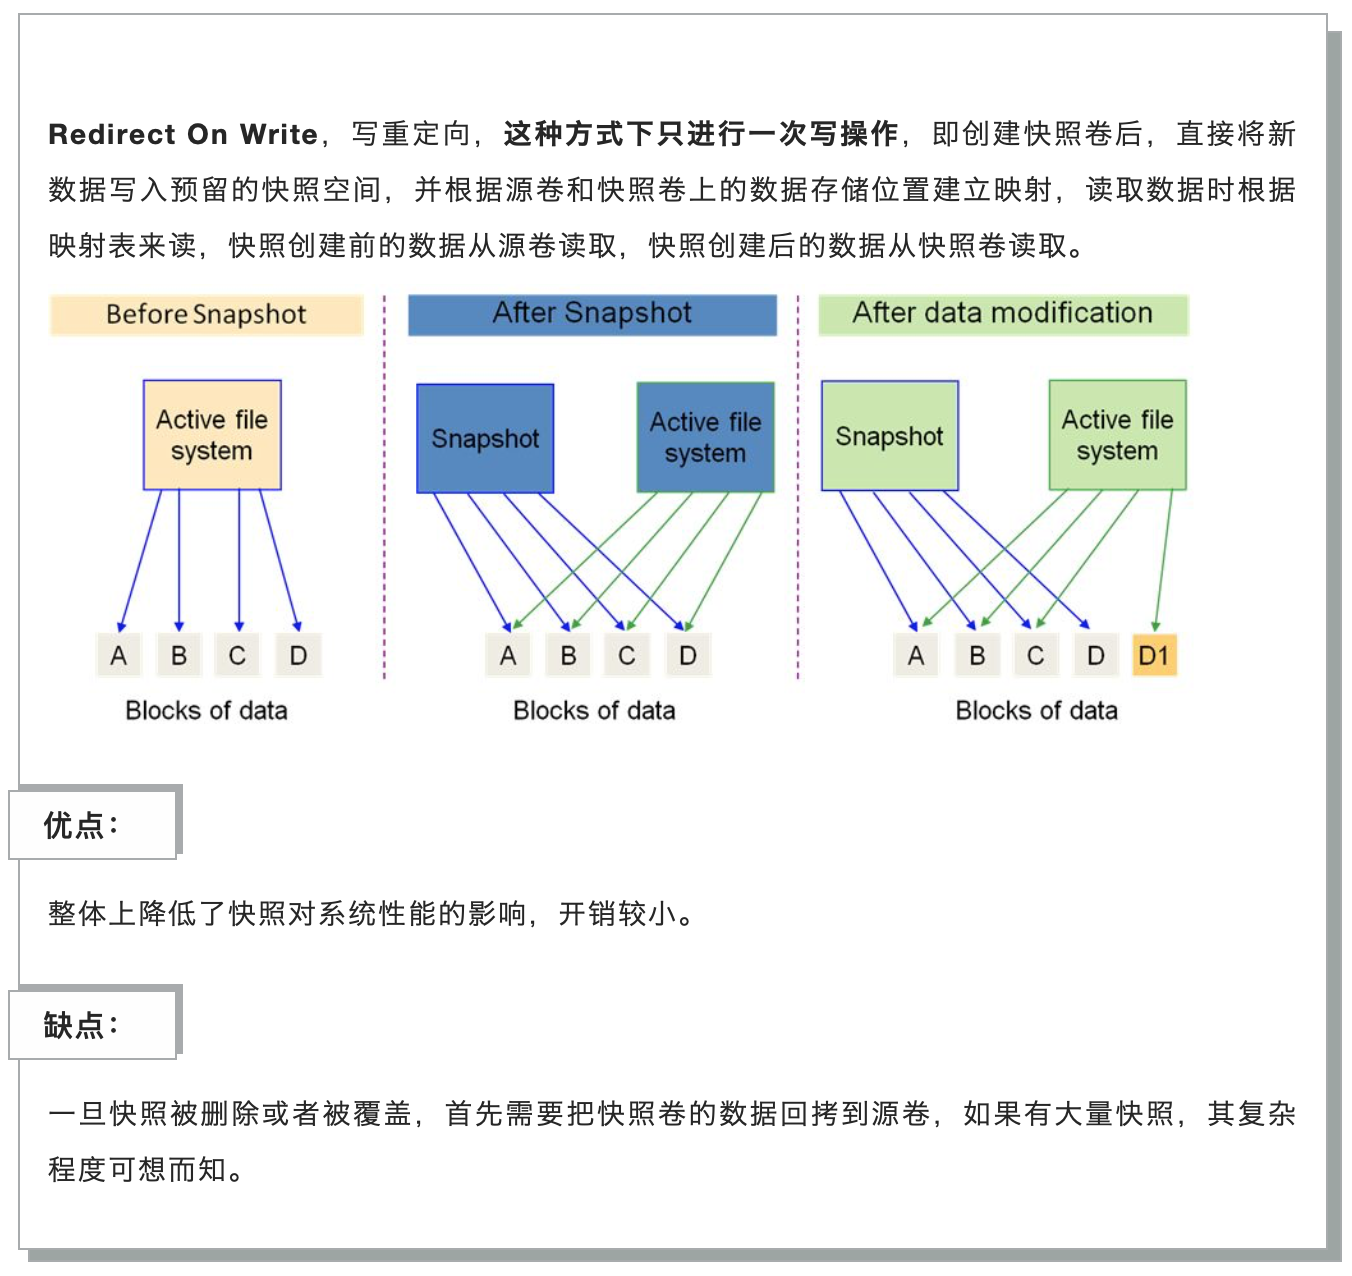
\includegraphics[height=11cm]{../imgs/row-snapshot.png}
\end{center}

如果发生卷ID变化,上层应用需要重新打开卷,影响较大。

\subsection{delete}

快照包含有增量数据,除了叶子快照,不能直接删除。

\subsection{list}

快照树,隐藏或显示删除的快照。

\subsection{rollback}

直接用目标快照的快照头替换卷的快照头。

回收卷私有数据

\subsection{clone}

读取snapshot的内容。读取卷和快照是同一个过程。

\begin{center}
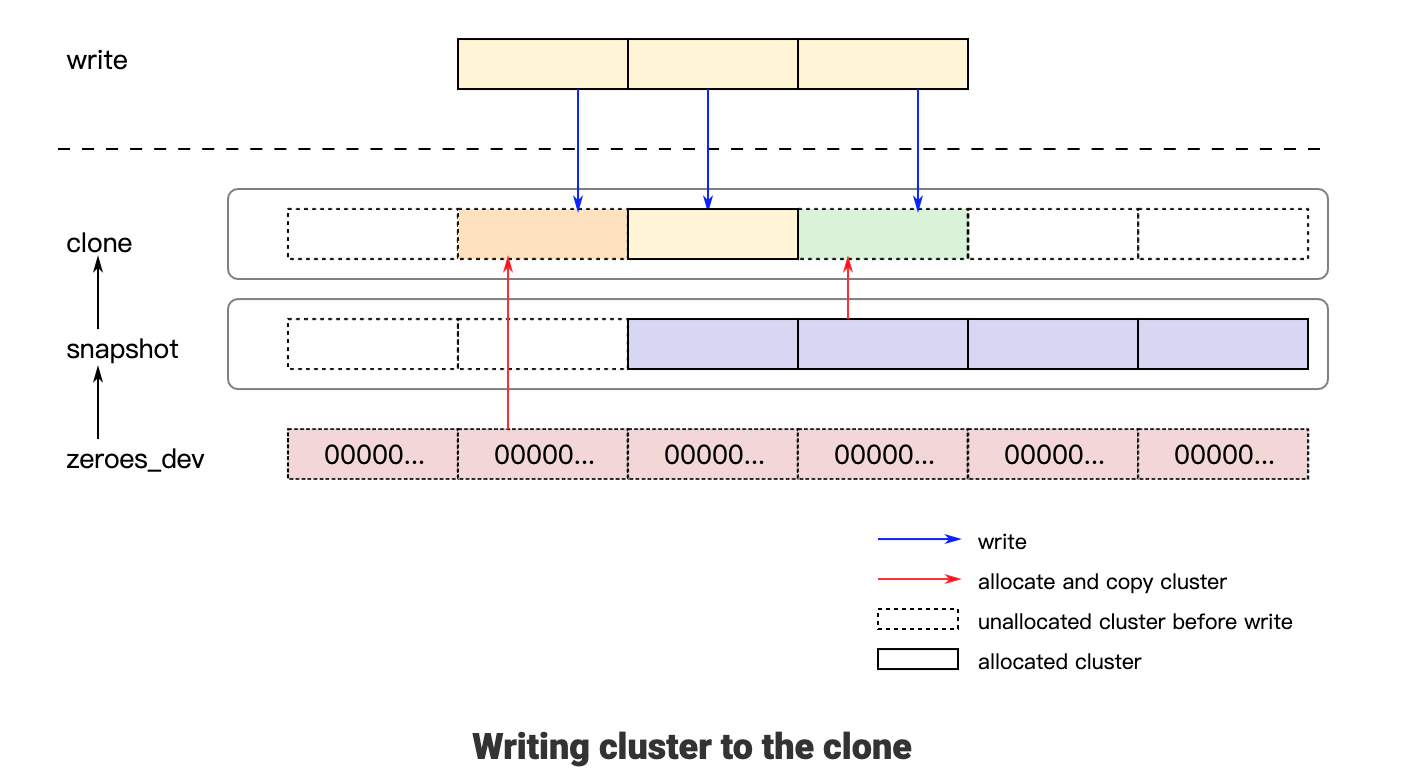
\includegraphics[width=11cm]{../imgs/clone-write.png}
\end{center}

\begin{center}
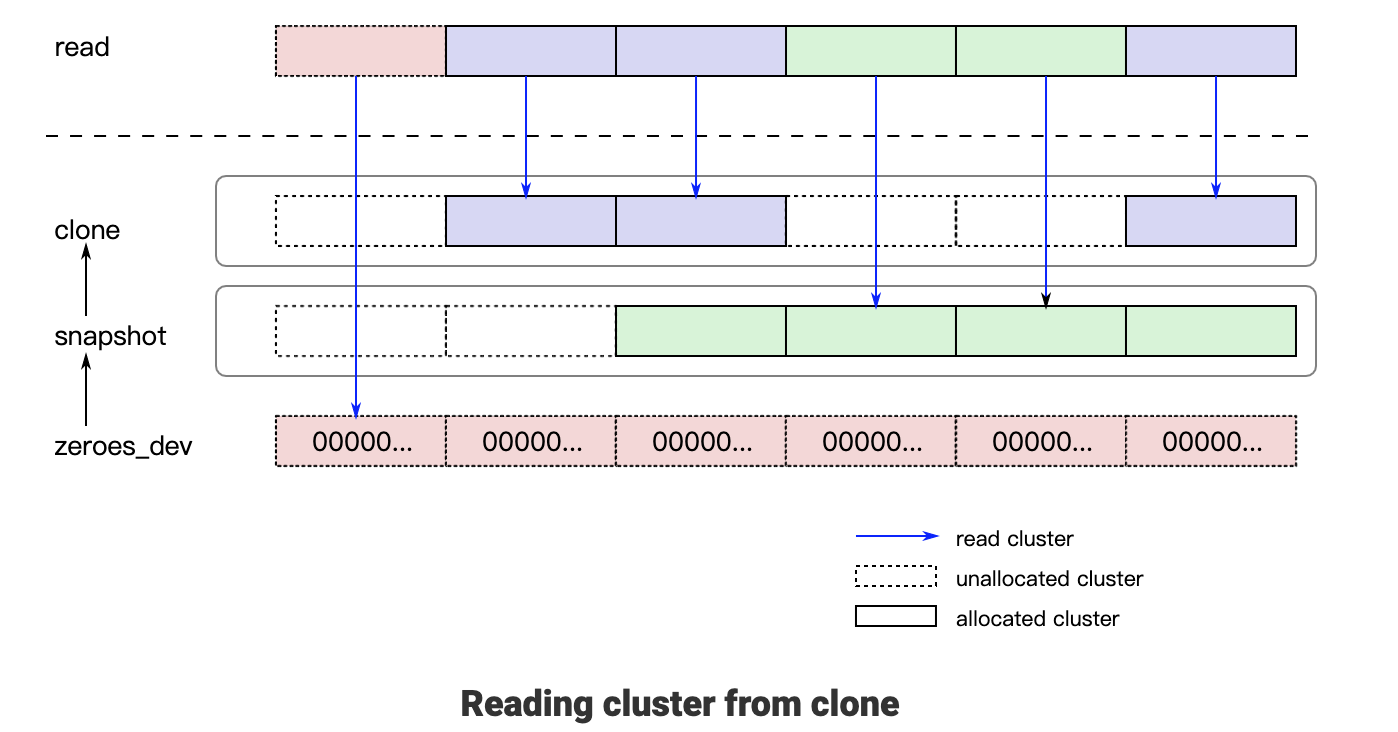
\includegraphics[width=11cm]{../imgs/clone-read.png}
\end{center}

\subsection{flatten}

\subsection{protect/unprotect}
